\documentclass{article}
\usepackage[french]{babel}
\usepackage[T1]{fontenc}
\usepackage[utf8]{inputenc}
\usepackage{graphicx} % Required for inserting images
\usepackage{mathtools}
\usepackage{listingsutf8}
\usepackage{amsfonts}
\usepackage{amssymb}
\lstset{%
    inputencoding=utf8,
    literate=
        {é}{{\'e}}{1}%
        {è}{{\`e}}{1}%
        {à}{{\`a}}{1}%
        {â}{{\^a}}{1}%
        {ç}{{\c{c}}}{1}%
        {œ}{{\oe}}{1}%
        {ù}{{\`u}}{1}%
        {É}{{\'E}}{1}%
        {È}{{\`E}}{1}%
        {À}{{\`A}}{1}%
        {Ç}{{\c{C}}}{1}%
        {Œ}{{\OE}}{1}%
        {Ê}{{\^E}}{1}%
        {ê}{{\^e}}{1}%
        {î}{{\^i}}{1}%
        {ï}{{\"i}}{1}%
        {ô}{{\^o}}{1}%
        {û}{{\^u}}{1}%
}
\usepackage{fullpage}
\usepackage[margin=2.1cm]{geometry}
\usepackage{setspace}
\usepackage{todonotes}
\usepackage{amsthm}

\newtheoremstyle{exostyle}% style name
{10pt}% above space
{10pt}% below space
{}% body font
{}% indent amount
{\scshape\bfseries\large}% head font
{\hfill\vspace{5pt}\newline}% post head punctuation
{0pt}% Space after theorem head
{\hfill\thmname{#1}\thmnumber{ #2} -- \thmnote{ #3}}% head spec

\newtheoremstyle{partiestyle}% style name
{1em}% above space
{1em}% below space
{}% body font
{}% indent amount
{\bfseries}% head font
{\vspace{.5em}\newline}% post head punctuation
{0em}% Space after theorem head
{\thmnumber{#2} \thmnote{ #3}}% head spec

\newtheoremstyle{questionstyle}% style name
{.5em}% above space
{.5em}% below space
{}% body font
{}% indent amount
{\bfseries}% head font
{}% post head punctuation
{0em}% Space after theorem head
{Question \thmnumber{#2 }}% head spec

\theoremstyle{exostyle}
\newtheorem{exo}{Exercice}

\theoremstyle{partiestyle}
\newtheorem{partie}{}[exo]

\theoremstyle{questionstyle}
\newtheorem{question}{Question}[exo]
\newtheorem{questionpartie}{Question}[partie]

\title{Examen terminal: Algorithmes}
\author{L1 MPCI}
\date{22 mai 2026 - Durée: 2h}

\begin{document}

\maketitle

\begin{center}
{\em On rappelle qu'aucun document, ni équipement électrique ou électronique n'est autorisé.

 {\bf Cependant} l'usage d'un coussin péteur sera toléré s'il est placé sur le siège d'un autre étudiant que soit-même.}
\end{center}


\vspace*{1cm}

\paragraph{Les exercices de cet examen} :
\begin{itemize}
\item sont au nombre de 2;
\item sont indépendants;
\item sont chacun constitués de parties de difficultés croissantes.
\end{itemize}


\paragraph{}{\large \sc Rendez \underline{des copies séparées pour chaque exercice}, ceci vous permettra de d'y revenir au cours de l'examen sans perdre le correcteur.}


\clearpage

\begin{exo}[Inversions]
    On considérera dans cet exercice des tableaux d'entiers $T$ de longueur $n$. On appelle \textit{inversion} un couple d'indices $(i, j)$ tel que  :
    \begin{itemize}
        \item $0 \leq i <  j < n$
        \item $T[i] >  T[j]$
    \end{itemize}
    Le but de cet exercice est de compter le nombre d'inversions d'un tableau donné. 
    \begin{partie}[Algorithmes naïfs]
        ~\vspace*{-.5cm}
        \begin{questionpartie}
            Combien d'inversions possède le tableau suivant : $T = [12, 2, 1, 2, 4, 1]$
        \end{questionpartie}
        \begin{questionpartie}
            Pour un tableau d'entiers de longueur $n$ quel est le nombre minimum et maximum d'inversions possibles ?
        \end{questionpartie}
        \begin{questionpartie}
            Démontrez que l'algorithme suivant rend le nombre d'inversions du tableau passé en paramètre et donnez sa complexité :
        \begin{tabbing}
            ccc\=cccc\=cccc\=cccc\=cccc\=cccc\=\kill
            \textbf{algorithme} \textsc{inversions}($T$: [entier]) $\rightarrow$ entier{\bf :}\\
            \>\vline$\,$ $nb \coloneqq \text{entier} \leftarrow 0$\\
            \>\vline$\,$ \textbf{pour chaque} $(i \coloneqq \text{entier})$ de $[0 .. T.\text{longueur}[$ {\bf :}\\
            \>\vline$\,$\>\vline$\,$ \textbf{pour chaque} $(j \coloneqq \text{entier})$ de $[0 .. T.\text{longueur}[$ {\bf :}\\
            \>\vline$\,$\>\vline$\,$ \>\vline$\,$ \textbf{si} $(i \leq j)$ \textbf{et} $(T[i] > T[j])$ {\bf :}\\
            \>\vline$\,$\>\vline$\,$\>\vline$\,$\>\vline$\,$ $nb \leftarrow nb + 1$\\
            \>\vline$\,$ \textbf{rendre} $nb$\\
        \end{tabbing}
        \vspace*{-.5cm}
        \end{questionpartie}
        \begin{questionpartie}
            Donnez le pseudo-code et la complexité d'un algorithme récursif de signature \texttt{\textsc{inversions\_rec}($T$: [entier], k: entier) $\rightarrow$ entier} qui rend le nombre d'inversions $(i, j)$ de $T$ telles que $j \leq k$.
        \end{questionpartie}
        \begin{questionpartie}
            Donnez le pseudo-code et la complexité d'un algorithme de signature \texttt{\textsc{inversions2}($T$: [entier]) $\rightarrow$ entier} utilisant l'algorithme récursif de la question précédente et rendant le nombre d'inversions du tableau passé en paramètre.
        \end{questionpartie}

    \end{partie}
    \begin{partie}[Un petit détour]
        On suppose que l'on possède deux tableaux d'entiers $T_1$ et $T_2$ de longueurs respectives $n_1$ et $n_2$ et on cherche à déterminer le nombre de couples $(i, j)$ tels que $T_1[i] > T_2[j]$ avec $0 \leq i < n_1$ et $0 \leq j < n_2$ (on peut avoir $j \leq i$ ici puisque l'on travaille sur 2 tableaux différents). 
        \begin{questionpartie}
            Donnez le pseudo-code d'un algorithme naïf de signature \texttt{\textsc{inversions\_entre\_tableaux}($T_1$: [entier], $T_2$: [entier]) $\rightarrow$ entier} et de complexité $\mathcal{O}(n_1 \cdot n_2)$ permettant de calculer ce nombre.
        \end{questionpartie}
        \begin{questionpartie}
            Montrez que si les tableaux $T_1$ et $T_2$ sont tous deux triés par ordre croissant, on peut faire mieux et calculer le nombre d'inversions entre $T_1$ et $T_2$ avec un algorithme de complexité $\mathcal{O}(n_1 + n_2)$ dont vous donnerez le pseudo-code. Il sera de signature \texttt{\textsc{inversions\_entre\_tableaux\_triée}($T_1$: [entier], $T_2$: [entier]) $\rightarrow$ entier}.
        \end{questionpartie}
    \end{partie}
    \begin{partie}[Un algorithme plus efficace]
        ~\vspace*{-.5cm}
        \begin{questionpartie}
            Donnez le pseudo-code et rappelez la complexité du tri fusion (pour simplifier, on supposera que la longueur $n$ du tableau à trier est une puissance de 2 : $n = 2^p$).
        \end{questionpartie}
        \begin{questionpartie}
            En reprenant l'idée du tri fusion donner le pseudo-code d'un algorithme récursif de complexité $\mathcal{O}(n\ln(n))$ (ce que, bien sûr, vous justifierez) permettant de rendre le nombre d'inversions d'un tableau $T$ de longueur $n$ (on supposera encore ici que $n$ est une puissance de 2). Cet algorithme sera de signature \texttt{\textsc{indices\_rec}($T$: [entier]) $\rightarrow$ ([entier], entier)} et rendra un couple constitué d'une copie triée de $T$ et du nombre d'inversions de $T$.
        \end{questionpartie}
    \end{partie}

\newpage

\end{exo}
\begin{exo}[Skip list]
    Le but de cet exercice est d'étudier la structure de donnée nommée \textit{skip list} définie en 1990 par  William Pugh\footnote{William Pugh, \textit{Skip lists: a probabilistic alternative to balanced trees}, Communications of the ACM, 33, 6 pp 668 - 676.}.
    \begin{partie}[Recherche et insertion dans une liste triée]
        ~\vspace*{-.5cm}
        \begin{questionpartie}
            Donnez le pseudo-code (et sa preuve bien sûr) et la complexité de l'algorithme de la recherche dichotomique dans un tableau d'entier trié. Votre algorithme devra être de signature : \texttt{\textsc{recherche\_dichotomique}($T$: [entier], $v$: entier) $\rightarrow$ booléen} et rendra vrai si $v$ est dans $T$ et faux sinon.
        \end{questionpartie}
        \begin{questionpartie}
            On remplace souvent les tableaux par la  structure de donnée \textbf{des listes}. Explicitez les différences entre les deux structures et pourquoi il est (presque) toujours plus avantageux d'utiliser des listes plutôt que des tableaux.
        \end{questionpartie}
        \begin{questionpartie}
            Donnez le pseudo-code et la complexité d'un algorithme ajoutant un élément dans une liste triée. Votre algorithme modifiera la liste passée en entrée et elle devra rester triée. Enfin,  la complexité spatiale de votre algorithme devra être en $\mathcal{O}(1)$ (vous ne comptez pas la complexité spatiale de la liste passée en paramètre).
        \end{questionpartie}
        \begin{questionpartie}
            Plutôt que d'utiliser des listes on peut aussi utiliser des listes doublement chaînées définies comme une succession de maillons.
            \label{struct-maillon}
            \begin{tabbing}
                ccc\=cccc\=cccc\=cccc\=cccc\=cccc\=\kill
                \textbf{structure} \textsc{maillon}{\bf :}\\
                \>\vline$\,$   valeur: T $\leftarrow \varnothing$\\
                \>\vline$\,$ précédent: Maillon $\leftarrow \varnothing$\\
                \>\vline$\,$ suivant: Maillon$\leftarrow \varnothing$\\
            \end{tabbing}
        \vspace*{-.5cm}
            Donnez le pseudo-code et la complexité minimale, maximale et en moyenne d'un algorithme ajoutant un élément dans une liste doublement chaînée triée avant et après l'ajout. 
        \end{questionpartie}
        \begin{questionpartie}
            Quels sont les avantages et inconvénients de ces deux structures pour rechercher/ajouter/supprimer des entiers dans une structure devant rester triée ?
        \end{questionpartie}
    \end{partie}
    \begin{partie}[\textit{Skip list} régulière]
        La figure~\ref{fig-sl-reg} montre une représentation d'une \textit{skip list} régulière.
        \begin{figure}[h!]
            \begin{center}
            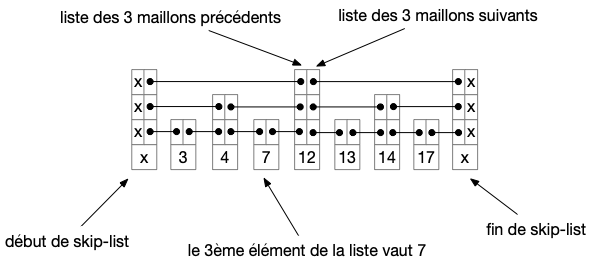
\includegraphics[scale=.45]{skip-list-régulière.png}
            \end{center}
            \caption{Une skip-list régulière.\label{fig-sl-reg}}
        \end{figure}
        Une \textit{skip list} est une généralisation d'une liste chaînée où chaque maillon possède une liste de maillons précédents et une liste de maillons suivants. Cette structure suit les règles suivantes :
        \begin{itemize}
            \item la longueur des listes suivants et précédents est la même pour un maillon donné et est appelée niveau (le deuxième élément de la figure~\ref{fig-sl-reg} possède 2 niveaux et le troisième élément 1 seul niveau)
            \item pour un maillon donné, le $i$ème élément de sa liste suivant (respectivement de sa liste précédent) vaudra le prochain (\textit{resp.} précédent) maillon de la liste de niveau $i$ ou plus.
            \item une skip list possède un premier maillon qui débute la liste et un maillon qui termine la liste. Ces deux maillons ne possèdent pas de valeurs et sont de niveau maximum noté $K$.
        \end{itemize}
        Une \textit{skip list} sera dite \textit{régulière} si le $i$ème élément de la liste ($1\leq i \leq n$) est de niveau $k+1$ avec $k$ le plus grand entier tel que $2^k$ divise $i$.

        \begin{questionpartie}
            Montrer que la figure~\ref{fig-sl-reg} représente une \textit{skip list} régulière.
        \end{questionpartie}

        \begin{questionpartie}
            Modifiez la structure de maillon de la question~\ref{struct-maillon} pour permettre de construire une structure \textsc{maillon\_sl} d'un maillon de \textit{skip list}.
        \end{questionpartie}
        \begin{questionpartie}
            Utilisez la structure que vous avez créée à la question précédente pour donner le pseudo-code d'un algorithme de signature \texttt{\textsc{crée\_maillon}($v$: entier, $k$: entier) $\rightarrow$ \textsc{maillon\_sl}} qui rendre un maillon de \textit{skip list} de niveau $k\geq 1$.
        \end{questionpartie}
        \begin{questionpartie}
            \label{recherche-sl}
            Donnez le pseudo-code et la complexité d'un algorithme cherchant une valeur dans une \textit{skip list}. Il devra être de signature \texttt{\textsc{recherche}($slr$: \textsc{maillon\_sl}, $v$: entier) $\rightarrow$ booléen} et rendra vrai si la valeur $v$ est présente dans la \textit{skip list} régulière $slr$ et faux sinon.
        \end{questionpartie}
        \begin{questionpartie}
            Donnez un argument qui justifie le fait que maintenir la structure de \textit{skip list} régulière dans le cas de l'ajout (respectivement la suppression) d'un élément nécessite au minimum de parcourir tous les éléments après l'élément ajouté (\textit{resp.} supprimé).
        \end{questionpartie}
        \begin{questionpartie}
            Déduisez des deux questions précédentes la complexité de la recherche, de l'ajout et de la suppression d'un élément dans une \textit{skip list} régulière.
        \end{questionpartie}

    \end{partie}
    \begin{partie}[\textit{Skip list} quelconque]
        Une \textit{skip list} ne spécifie pas le nombre de maillons suivants que doit posséder un élément. La figure~\ref{fig-sl} représente une \textit{skip list} valide. Lors de l'ajout d'un élément dans la \textit{skip list} son niveau $k$ est déterminé par l'algorithme \texttt{\textsc{nombre}} qui utilise la fonction \texttt{\textsc{random}() $\rightarrow$ réel} qui rend un réel aléatoire choisi uniformément dans $[0, 1]$.

        \begin{figure}[h!]
            \begin{center}
            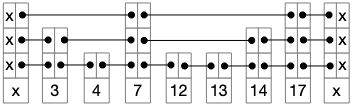
\includegraphics[scale=.45]{skip-list.png}
            \end{center}
            \caption{Une skip-list.\label{fig-sl}}
        \end{figure}

            \begin{tabbing}
                ccc\=cccc\=cccc\=cccc\=cccc\=cccc\=\kill
                \textbf{algorithme} \textsc{nombre}($K$: entier) $\rightarrow$ entier{\bf :}\\
                \>\vline$\,$  $k$:= entier $\leftarrow 1$\\
                \>\vline$\,$ \textbf{tant que} $(k < K)$ \textbf{et} \textsc{random()}$\leq 1/2$ {\bf :}\\
                \>\vline$\,$\>\vline$\,$ $k$ $\leftarrow k + 1$\\
                \>\vline$\,$ \textbf{rendre} $k$ \\
            \end{tabbing}
        \vspace*{-.5cm}
        \begin{questionpartie}
            Donnez la complexité minimale et maximale de l'algorithme de la question~\ref{recherche-sl} appliqué à une \textit{skip list} quelconque.
        \end{questionpartie}
        \begin{questionpartie}
            Donnez le pseudo-code d'un algorithme insérant une valeur dans une \textit{skip list}.
        \end{questionpartie}
    \end{partie}
    \begin{partie}[Estimation des complexités moyennes]
        ~\vspace*{-.5cm}
        \begin{questionpartie}
            Pour une \textit{skip list} donnée, combien y a-t-il en moyenne de maillons de niveau $k$ ?
            % proba 1/2 d'être de niveau 1 et proba 1-1/2 d'être de niveau > 1 et on récurse.
            % proba 1 = 1/2 ; proba 2 = (1-1/2) * 1/2 ; ... ; proba i 1/2^i
        \end{questionpartie}
        \begin{questionpartie}
            Pour une \textit{skip list} donnée, combien y a-t-il en moyenne de maillons de niveau strictement inférieur à $k$ entre 2 maillons successifs de niveau $k$ ou plus ?
            % si k ou plus il a fallu arriver à k-1. Parmi tous ceux à k-1 seule la moitié est monté en k : il y a autant de k-1 exactement que de >= k : il y a en moyenne 1 de niveau k-1 entre 2 de niveau k ou plus
            % 1 maillon de niveau k-1 entre 2 maillons successifs de niveau k ou plus. Car monter d'un niveau est de proba 1/2
        \end{questionpartie}
        \begin{questionpartie}
            Estimez la complexité en moyenne de l'algorithme de la question~\ref{recherche-sl} appliqué à une \textit{skip list} quelconque.
        \end{questionpartie}
        \begin{questionpartie}
            Si vous aviez $n$ éléments à stocker dans une \textit{skip list}, quelle valeur donneriez vous (et pourquoi) à son niveau maximum $K$ ?
        \end{questionpartie}
    \end{partie}
    % \begin{partie}[Calcul des complexités]
    %         % ajouter partie pour l'étude rigoureuse avec des listes infinies et une proba p. Voir papier original. https://dl.acm.org/doi/pdf/10.1145/78973.78977

    %     % Cas général avec $p$ plutôt que 1/2.
    %     \begin{questionpartie}
    %     \end{questionpartie}
    % \end{partie}


    % \url{https://www.youtube.com/watch?v=HIrh1NJmQxM}
    % \url{https://courses.cs.umbc.edu/undergraduate/341/fall01/Lectures/SkipLists/skip_lists/skip_lists.html}



\end{exo}
% \begin{exo}[Filtre de Bloom]
% peut-être.
% \end{exo}

\end{document}